%%
\begin{table}[htdp]
\caption[The Gram-Schmidt orthogonalization process for two vectors]{The Gram-Schmidt orthogonalization process is detailed for the two input vectors in the previous table. Pick an ordering to sweep through the set of vectors since the process is order dependent. The first action is to normalize the length of the first vector as shown in step 1. Find the orthogonal projection of the second vector onto the first vector. This projection is shown with the red arrow in step 2. For the next step, subtract this projection from the second vector which ``straightens up'' this vector as shown in step 3. Finally, normalize the new vector as shown in step 4.}
\begin{center}
\begin{tabular}{cc}
%
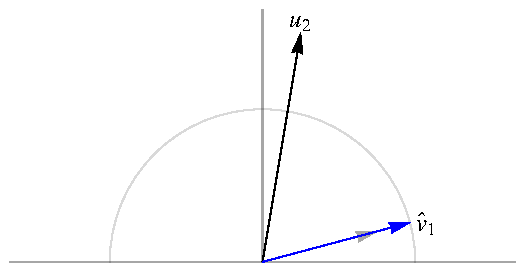
\includegraphics[ width = 2.25in ]{images/appendices/"gram schmidt"/gs_01.pdf} &
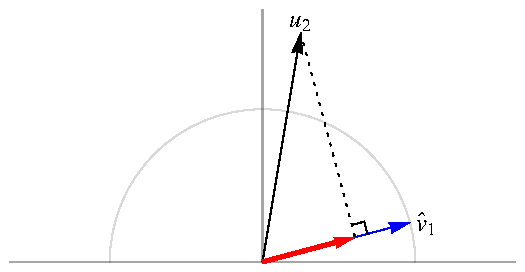
\includegraphics[ width = 2.25in ]{images/appendices/"gram schmidt"/gs_02.pdf} \\
%
\text{Step 1: normalization of $v_{1}$.} &
\text{Step 2: projection onto $v_{1}$.} \\[10pt]\hline
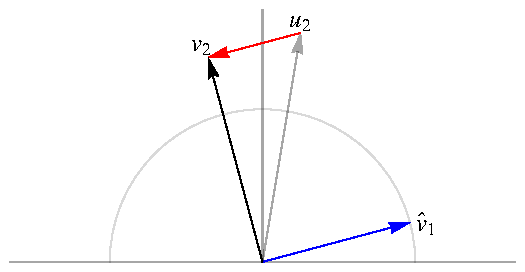
\includegraphics[ width = 2.25in ]{images/appendices/"gram schmidt"/gs_03.pdf} &
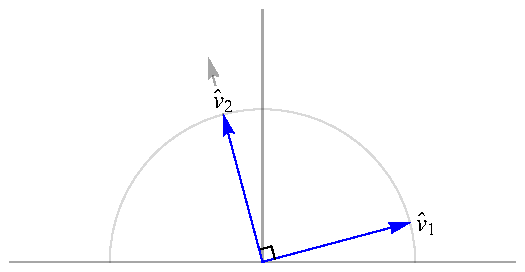
\includegraphics[ width = 2.25in ]{images/appendices/"gram schmidt"/gs_04.pdf} \\
%
\text{Step 3: subtract projection.} &
\text{Step 4: normalization of $v_{2}$.}  
%
\end{tabular}
\end{center}
\label{tab:gs:guts}
\end{table}

\endinput